\chapter{Explainability in Reinforcement Learning}
\label{chap:explainability_in_reinforcement_learning}

\chapterepigraph{The Answer to the Great Question\ldots{} Of Life, the Universe and Everything\ldots{} Is\ldots{} Forty-two.}
{Douglas Adams, \textit{The Hitchhiker's Guide to the Galaxy} (1979)~\parencite{adams1979hitchhiker}}

\glsresetall

Today, the majority of \gls{ai} agents with which humans interact are deployed in controlled or low-risk environments.
For example, agents capable of playing games such as Go operate in settings where potential errors remain limited in terms of consequences \parencite{silver2017mastering}.
Even more autonomous systems, such as agents based on \glspl{llm}, remain constrained by human supervision mechanisms and are often restricted to tasks such as code generation or information retrieval \parencite{chen2021evaluating, lewis2021retrievalaugmentedgenerationknowledgeintensivenlp}.

Safety-critical applications integrating machine learning components are still rare.
Introducing autonomous agents in such environments, requires the establishment of strong guarantees \parencite{seshia2022toward}.
These requirements include in particular:
\begin{itemize}
    \item validating the system's functioning before deployment,
    \item identifying the origin of a malfunction in case of failure,
    \item and certifying that an observed failure will not occur again.
\end{itemize}

The main challenge lies in the fact that the performing agents currently available rely on both \gls{rl} and \gls{dl} \parencite{mnih2013playingatarideepreinforcement}.
As a result, the mechanisms underlying their decisions cannot be understood directly from the learned model.
This lack of explainability makes their use difficult in safety-critical contexts.

To address this limitation, the field of \gls{xrl} has emerged as a subfield of \gls{xai}.
The objective of \gls{xrl} is to develop explainability methods that make it possible to obtain explanations of \gls{rl} agents.
Due to the relevance of the topic and to foster broader real-world adoption of \gls{rl}, a growing number of research teams are working on developing new explainability methods.
This enthusiasm is reflected in a rapid increase in the number of publications, as illustrated in Figure~\ref{fig:count_publications_xrl}.\footnote{The algorithm used to retrieve and match the arXiv papers is available at \url{https://github.com/Maxalaar/ArXiv_Papers_Matching}. The complete search protocol, including the databases consulted and the full set of query terms, has been archived on Zenodo \url{https://zenodo.org/records/19387785}.}

\begin{figure}[t]
    \centering
    \resizebox{0.9\textwidth}{!}{
    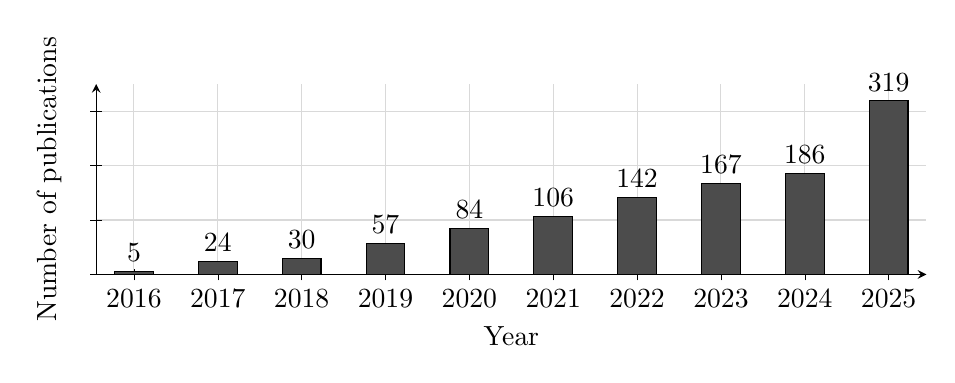
\begin{tikzpicture}
    \begin{axis}[
        width=\linewidth,
        height=4cm,
        ybar,
        bar width=14pt,
        ymin=0,
        ymax=350,
        yticklabels={},
        ylabel={Number of publications},
        xlabel={Year},
        symbolic x coords={2016,2017,2018,2019,2020,2021,2022,2023,2024,2025},
        nodes near coords,
        nodes near coords align={vertical},
        grid=both,
        major grid style={gray!30},
        minor grid style={gray!15},
        axis lines=left,
        tick style={black},
        enlarge x limits=0.05,
        title style={font=\bfseries},
    ]
    \addplot[
        fill=black!70
    ] coordinates {
        (2016,5)
        (2017,24)
        (2018,30)
        (2019,57)
        (2020,84)
        (2021,106)
        (2022,142)
        (2023,167)
        (2024,186)
        (2025,319)
    };
    \end{axis}
    \end{tikzpicture}
    }
    \caption{Yearly growth of \glsfmtshort{xrl} research with at least one citation on arXiv.}
    \label{fig:count_publications_xrl}
\end{figure}


The growing number and diversity of these methods make it increasingly difficult to obtain a unified view of the field.
This motivated our work on developing a unified taxonomy of explainability methods for \gls{rl}, initially presented in \parencite{alaarabiou:hal-04685607}.
The taxonomy provides a common structure for organizing existing approaches according to the type of information they use and the form of explanation they provide.
Building on this work, this chapter provides a detailed presentation of the proposed taxonomy and uses it to organize a broader state-of-the-art review of \gls{xrl}.

This chapter is organized as follows:
\begin{itemize}
    \item Section~\ref{sec:explainability_in_reinforcement_learning_explanation_in_artificial_intelligence} begins by clarifying what we mean by an explanation in the context of \gls{xai}.
    \item Section~\ref{sec:explainability_in_reinforcement_learning_explanation_in_artificial_intelligence} then introduces a taxonomy for categorizing existing \gls{xrl} methods.
    \item Section~\ref{sec:explainability_in_reinforcement_learning_state_of_the_art_review_of_xrl_methods} provides a comprehensive state-of-the-art review structured around this taxonomy.
    \item Section~\ref{sec:explainability_in_reinforcement_learning_conclusion} concludes the chapter with a summary and discussion.
\end{itemize}

\section{Explanation in Artificial Intelligence}
\label{sec:explainability_in_reinforcement_learning_explanation_in_artificial_intelligence}

In this section, we define what an explanation is in the context of \gls{xai} and how it can be obtained.
We first introduce the concept of explanation in general.
We then describe how this concept applies to \gls{xai}.
Finally, we further detail the properties that characterize an explainability method in the context of \gls{xai}.

\subsection{Explanation}
\label{subsec:explanation}
Defining what constitutes an explanation is challenging because the concept is inherently multidisciplinary.
When we refer to explanation, we are inherently referring to an explanation provided to a human.
As soon as humans are involved, the problem is no longer purely mathematical.
It involves several fields of research, such as philosophy, psychology, and sociology.
So far, these disciplines have not converged on a unified definition of explanation that can be directly applied to \gls{xai} \parencite{miller2019explanation, bellucci2021towards}.

For this reason, we propose the following definition of explanation.
An explanation involves two entities: the object (Definition~\ref{def:object}) being explained and the receiver of the explanation.
The receiver is a human who aims to understand how the object operates and will be referred to as the observer throughout this thesis (Definition~\ref{def:observer}).
The observer seeks to understand the object and, in doing so, builds a mental model of its functioning.

An explanation is therefore what allows the observer to refine and correct their mental model of how the object operates (Definition~\ref{def:explanation}).
This refinement is obtained through a transformation process that produces an explanation from the object being explained.
We refer to this process as an explainability method (Definition~\ref{def:explainability_method}), detailed further in Section~\ref{subsec:explainability_method}.
For an observer to understand an explanation, the information it contains must be interpretable (Definition~\ref{def:interpretable}).
Information is considered interpretable when it can be directly understood by a human without requiring any additional transformation process.

\begin{definition}{Object}{object}
The object of an explanation is the system the observer wants to understand.
\end{definition}

\begin{definition}{Observer}{observer}
The observer is the human who aims to understand an object.
The observer possesses a mental model of the object being explained.
This mental model is an internal representation of how the observer believes the system operates.
This representation may be incomplete or inaccurate.
\end{definition}

\begin{definition}{Interpretable}{interpretable}
Information is interpretable when it can be directly understood by an observer without requiring any additional transformation process.
\end{definition}

\begin{definition}{Explanation}{explanation}
An explanation is any interpretable information that enables an observer to refine or correct their mental model of the object of the explanation.
\end{definition}

\begin{definition}{Explainability Method}{explainability_method}
An explainability method is a transformation process that produces an explanation from the object being explained.
\end{definition}

Figure~\ref{fig:explanation_process_illustration} summarizes this whole explanation process, from the object of the explanation to the mental model refined by the observer, as a chain of three information structures, depicted as boxes and connected by arrows denoting a transformation of information:
\begin{enumerate}
    \item[(1)] The object of the explanation, that is, the system the observer seeks to understand.
    \item[(2)] The explanation, the interpretable information produced from the object.
    This transformation is performed through the use of an explainability method.
    \item[(3)] The mental model held by the observer regarding the object.
\end{enumerate}
A brace spanning boxes~(2) and~(3) indicates that this second half of the process, from the explanation to the resulting mental model, constitutes a subjective analysis carried out by the observer.

\begin{figure}[t]
    \centering

    % --- Layout parameters --------------------------------------------
    % Horizontal distance between the centers of two consecutive blocks.
    \pgfmathsetmacro{\blockDistance}{6.6}
    % Width/height of each block (keep in sync with the node styles below).
    \pgfmathsetmacro{\blockSize}{3.6}
    % Fixed text width inside each block, so that longer labels wrap onto
    % extra lines (growing the block downward) instead of growing wider
    % and colliding with the neighboring block.
    \pgfmathsetmacro{\blockTextWidth}{3.1}
    % Text width used for the labels placed above/below the arrows.
    \pgfmathsetmacro{\arrowTextWidth}{2.6}
    % Diameter of the step-number badges pinned to each block's corner.
    \pgfmathsetmacro{\badgeSize}{0.65}

    % Vertical offset of the legend row below the main diagram.
    \pgfmathsetmacro{\legendYShift}{-3.6}
    % Horizontal offset of the start of the legend row (position of its first icon).
    \pgfmathsetmacro{\legendXShift}{-\blockSize/2 + 0}
    % Horizontal gap between two consecutive legend entries.
    \pgfmathsetmacro{\legendGap}{1.5}
    % Horizontal gap between a legend icon and its own label.
    \pgfmathsetmacro{\legendIconTextGap}{0.3}
    % --------------------------------------------------------------------

\resizebox{\textwidth}{!}{
\begin{tikzpicture}[]
% Nodes
\node[draw, rectangle, align=center, text width=\blockTextWidth cm, minimum width=\blockSize cm, minimum height=\blockSize cm] (box1) at (0, 0) {\hyperref[def:object]{\hl{\textbf{Object}}} \\ the system \\ the observer \\ seeks to understand};
\node[draw, rectangle, right of=box1, align=center, text width=\blockTextWidth cm, minimum width=\blockSize cm, minimum height=\blockSize cm] (box2) at (\blockDistance, 0) {\hyperref[def:explanation]{\hl{\textbf{Explanation}}} \\ \hyperref[def:interpretable]{\hl{interpretable}} \\ information enabling \\ the observer to refine \\ their mental model};
\node[draw, rectangle, right of=box2, align=center, text width=\blockTextWidth cm, minimum width=\blockSize cm, minimum height=\blockSize cm] (box3) at (2*\blockDistance, 0) {\textbf{Mental model} \\ of the observer \\ regarding the object};
% Step numbers: small badges pinned to the top-left corner of each box, so
% the figure can be referenced step by step from the surrounding text.
\node[circle, draw, fill=white, font=\bfseries\large, inner sep=0pt, minimum size=\badgeSize cm] at (box1.north west) {1};
\node[circle, draw, fill=white, font=\bfseries\large, inner sep=0pt, minimum size=\badgeSize cm] at (box2.north west) {2};
\node[circle, draw, fill=white, font=\bfseries\large, inner sep=0pt, minimum size=\badgeSize cm] at (box3.north west) {3};
% Arrows
\draw[-{Latex[length=3mm]}] (box1) -- node[midway, above, align=center, text width=\arrowTextWidth cm] {Information \\ extraction \\ through the use \\ of an \\ \hyperref[def:explainability_method]{\hl{\textbf{explainability}\\\textbf{method}}}} node[midway, below, align=center] {} (box2);
\draw[-{Latex[length=3mm]}] (box2) -- node[midway, above, align=center, text width=\arrowTextWidth cm] {\textbf{Interpretation} \\ by \\ the observer} node[midway, below, align=center] {} (box3);

% Legend: each entry is chained to the previous one via \legendGap /
% \legendIconTextGap, so the whole row reflows consistently if a label
% changes length or if the gaps are retuned.
\node[draw, rectangle, minimum width=0.3cm, minimum height=0.3cm] (legendIcon1) at (\legendXShift, \legendYShift) {};
\node[anchor=west, right=\legendIconTextGap of legendIcon1] (legendText1) {Information structures};

\node[inner sep=0pt, anchor=west, right=\legendGap of legendText1] (legendArrowStart) {};
\coordinate (legendArrowEnd) at ([xshift=0.4cm]legendArrowStart);
\draw[-{Latex[length=1.5mm]}] (legendArrowStart) -- (legendArrowEnd);
\node[anchor=west, right=\legendIconTextGap of legendArrowEnd] (legendText2) {Information transformation};

\node[anchor=west, right=\legendGap of legendText2] (legendIcon3) {\hl{~~}};
\node[anchor=west, right=\legendIconTextGap of legendIcon3] (legendText3) {Concepts discussed in this section};

% Brace: spans from just past box2 to just past box3, so it automatically
% follows \blockDistance and \blockSize instead of being retuned by hand.
\coordinate (C) at (\blockDistance+\blockSize/2+1, 2.6);
\coordinate (D) at (2*\blockDistance+\blockSize/2+1, 2.6);
\draw [decorate, decoration={brace, amplitude=10pt}, thick]
          (C) -- node[above=12pt, align=center] {Subjective analysis \\ by the \hyperref[def:observer]{\hl{observer}}} (D);
\end{tikzpicture}
    }
\caption{Explanation process.}
\label{fig:explanation_process_illustration}
\end{figure}


This definition of explanation establishes the approach to explainability adopted throughout this thesis.
Under this definition, explainability is regarded as a continuum that evolves as knowledge develops \parencite{Siegel_Craver_2024, zednik2019solving}.

This quantitative perspective highlights that not all explanations provide the same level of value \parencite{doshivelez2017rigorous}.
The effectiveness of an explanation depends on its ability to improve the observer's understanding of the system.
For example, describing a marginal aspect of a system is different from correcting an observer's misunderstanding of a key mechanism.

\subsection{Explainable Artificial Intelligence}
\label{subsec:explainable_artificial_intelligence}

Now that the general framework of explanation has been established, we can examine how this concept applies in the context of \gls{ai}.
In the context of \gls{xai}, the object of explanation is an \gls{ai} system.
More precisely, \gls{xai} emerged as a response to the success of \gls{dl} models \parencite{gunning2019darpa, arrieta2020explainable}.
Unlike symbolic approaches, individual components of \glspl{nn} cannot be directly associated with human concepts.
From this starting point, we identify two types of approaches:
\begin{itemize}
    \item \textbf{Substitutive explainability:} In this approach, the assumption is that there is nothing to explain within a \gls{nn}.
    There is no semantic meaning associated with each computational component, and therefore nothing to interpret.
    This corresponds to the \enquote{black box} view of \glspl{nn}.
    Under this assumption, \gls{xai} consists of replacing as much of the \gls{dl} system as possible with alternative \gls{ai} methods \parencite{rudin2019stop}.

    \item \textbf{Intrinsic explainability:} In this approach, it is argued that \glspl{nn} contain mechanisms that can be explained.
    The limitation is considered to be the absence of adequate tools to analyze their functioning \parencite{olah2020zoom}.
\end{itemize}

This thesis considers methods from both approaches in order to provide a comprehensive overview of the \gls{xai} field.
However, it primarily adopts the perspective of the \MechanisticHypothesisName \parencite{Siegel_Craver_2024, zednik2019solving}.
Since this hypothesis assumes that the internal computations of a model can be explained, adopting it necessarily places this thesis within intrinsic explainability.
This perspective is more closely aligned with the definition of explainability adopted in this thesis, which considers explainability as a continuum that evolves with the development of knowledge.

\begin{hypothesis}{Mechanistic Hypothesis}{mechanistic}
Every \gls{ai} system results from a sequence of causal computations.
Because the rules governing these interactions are mechanical, the behavior of the system can be explained.
If an \gls{ai} system cannot be explained, this reflects a limitation of knowledge rather than an intrinsic property of the system.
\end{hypothesis}

The approach based on this hypothesis is generally called mechanistic interpretability in the literature \parencite{olah2020zoom}.
In this thesis, we refer to it as \gls{me} (Definition~\ref{def:mechanistic_explainability}).
The internal mechanisms of a \gls{nn} are indeed not interpretable in the sense of Definition~\ref{def:interpretable}, since an observer cannot understand them directly.
They only become understandable once an explainability method (Definition~\ref{def:explainability_method}) has transformed them into explanations (Definition~\ref{def:explanation}).
This approach therefore falls within explainability rather than interpretability.

\subsection{Explainability Methods}
\label{subsec:explainability_method}

Now that the general framework of \gls{xai} has been established, we need to further detail the properties of an explanation in this context.
In our framework, an explanation in the field of \gls{xai} can be characterized by three components:
\begin{itemize}
    \item \textbf{Source:}\label{item:source} refers to the origin of the information used by the explainability method.
    The explainability method transforms the raw information produced by the \gls{ai} system into an explanation that can be understood by an observer.

    \item \textbf{Form:}\label{item:form} refers to the representation through which the explanation is communicated.
    The form defines how the information is presented to the observer and must allow human interpretation.
    An explanation can take many different forms, including text, images, computer code, and mathematical equations.

    \item \textbf{Subject:}\label{item:subject} refers to the aspect of the \gls{ai} system that is being explained.
    In \gls{xai}, this distinction is commonly associated with the difference between local and global explanations.
    A local explanation describes why an \gls{ai} system produced a specific output in a given situation.
    A global explanation aims to describe the general functioning of the \gls{ai} system.
\end{itemize}

\section{Taxonomy of XRL Methods}
\label{sec:explainability_in_reinforcement_learning_taxonomy_of_xrl_methods}

Now that the concept of \gls{xai} has been defined, we turn to its application in \gls{rl}, known as \gls{xrl}.
As in \gls{xai}, explanations in \gls{xrl} are produced by explainability methods and can be described in terms of their subject, source, and form.
This section reviews the possible variations of these three aspects in the specific context of \gls{rl}.

\subsection{Subject}
\label{subsec:subject}

The first question to address is the subject of explanation in the context of \gls{rl}.
To answer this question, it is necessary to identify the different components involved in a \gls{rl} system and determine which of them constitutes the object of explanation.
A \gls{rl} system can be described through two main components: the environment and the policy.

The environment defines the dynamics in which the agent evolves, including the possible states, observations, actions, and transitions.
Environments are simulations designed by humans, and their dynamics are explicitly defined.
Therefore, it is assumed that the environment is known to the observer and does not require explanation.

The main object of interest is therefore the agent's policy.
The policy represents the decision-making mechanism of the agent.
It is a function that maps observations to actions and is learned through interaction with the environment in order to maximize the expected cumulative reward.
The policy is the component that encodes the learning process and that \gls{xrl} aims to explain.

Explaining a policy introduces additional challenges compared with classical \gls{xai} settings.
In traditional \gls{xai} problems, the objective is to explain an isolated decision, such as determining which features of an image led to a classification result.
In contrast, \gls{rl} introduces a temporal dimension into the decision-making process.
An action is not only determined by the current observation but also influences future states and rewards.
Therefore, understanding the behavior of an agent may require considering a sequence of interactions between the agent and its environment.

This temporal dimension leads to a distinction between two objectives of explanation in \gls{xrl}:
\begin{itemize}
    \item \textbf{Decision explanations:} focus on identifying the elements of the current observation that influenced the action selected by the policy.
    This type of explanation is close to classical \gls{xai} approaches, as it analyzes the relationship between inputs and outputs while abstracting away the sequential nature of the decision process.

    \item \textbf{Strategy explanations:} aim to characterize the agent's behavior over time.
    They focus on sequences of decisions and interactions with the environment in order to understand how the agent achieves its long-term objective.
    This type of explanation is specific to \gls{rl}, as it addresses the temporal and goal-oriented nature of the learning process.
\end{itemize}

These two objectives should not be considered as strictly separated categories, but rather as two extremes of a continuum.
Understanding the elements of an observation that influence a specific decision can help the observer generalize this information to infer broader aspects of the agent's behavior.
Conversely, understanding the agent's overall strategy can provide insights into the reasoning behind individual decisions.

\subsection{Source}
\label{subsec:source}

We identify three sources of explanation in \gls{rl}, all obtained during or after the learning process and containing information about the agent:
\begin{itemize}
    \item \textbf{Policies:} policies are functions that generate a distribution over the action space for a given observation.
    The objective of \gls{rl} is to learn a policy that maximizes the expected cumulative future rewards.
    During the learning phase, the policy is iteratively improved through interactions with the environment.

    \item \textbf{Trajectories:} trajectories represent sequences of successive interactions between the agent and the environment.
    At each step, the agent selects an action based on its observation, which modifies the environment and produces a reward as well as a new observation.
    This process continues until the end of the trajectory.

    \item \textbf{Value functions:} value functions provide predictions about the future outcome of a trajectory from a given observation.
    The most commonly used value function is the critic function, which estimates the expected sum of future rewards.
    This prediction guides the learning process, as the agent updates its policy to maximize the estimated future return.
    However, other types of value functions can also be used as sources of explainability.
\end{itemize}

\subsection{Form}
\label{subsec:form}

We identify six forms of explanation in the \gls{rl} setting:
\begin{itemize}
    \item \textbf{Policy Model:} an interpretable model of the agent's policy function.
    
    \item \textbf{Saliency Map:} a weighting of the input features representing their influence on the output of the policy function.
    
    \item \textbf{Counterfactual:} a modified observation obtained by perturbing the original observation in order to produce a different action from the agent.
    
    \item \textbf{Agent Trajectory:} a sequence of successive interactions between the agent and the environment.
    
    \item \textbf{Trajectory Prediction:} a prediction about the future evolution of the trajectory produced by a value function.
    
    \item \textbf{Interaction Model:} an interpretable model of the interactions between the agent and the environment.
\end{itemize}

Among the three components characterizing an explanation, the form is the one that varies most significantly across explainability methods.
While subjects and sources tend to be relatively stable in the \gls{xrl} literature, the diversity in how explanations are presented is considerably greater.
The list above is by no means definitive and may evolve as new approaches emerge.
For this reason, the following section is organized according to the form of explanations and presents existing explainability methods based on this criterion.

% The full title is too wide for the running head, which gets a shorter one.
\let\OriginalSectionMark\sectionmark
\renewcommand{\sectionmark}[1]{\OriginalSectionMark{Review of Explainability Methods}}
\section{State-of-the-Art Review of Explainable Reinforcement Learning Methods}
\label{sec:explainability_in_reinforcement_learning_state_of_the_art_review_of_xrl_methods}
\let\sectionmark\OriginalSectionMark

The purpose of this section is to detail the functioning of existing explainability methods (see Table~\ref{tab:taxonomy_methods}).
They are presented according to the form of explanation they produce, following the taxonomy introduced in Section~\ref{sec:explainability_in_reinforcement_learning_taxonomy_of_xrl_methods}.

\begin{table*}[t]
\hspace*{\fill}
\resizebox{\textwidth}{!}{
\begin{tblr}{|Q[c,m]|Q[c,m,4cm]|Q[c,m,7cm]|Q[c,m]|Q[c,m]|Q[c,m]|}
    \hline
    \SetCell[r=2]{c} \hyperref[subsec:subject]{\textbf{Explanation \\ Subject}} & \SetCell[r=2]{c} \hyperref[subsec:form]{\textbf{Explanation \\ Form}} & \SetCell[r=2]{c} \hyperref[sec:explainability_in_reinforcement_learning_state_of_the_art_review_of_xrl_methods]{\textbf{Explainability \\ Method Family}} & \SetCell[c=3]{} \hyperref[subsec:source]{\textbf{Source of \\ Explanation}} & & \\
    \hline
    & & & \rotatebox{-90}{\shortstack{Policy}\hspace*{2mm}} & \rotatebox{-90}{\shortstack{Trajectories}\hspace*{2mm}} & \rotatebox{-90}{\shortstack{Value \\ functions}\hspace*{2mm}} \\
    \hline
    \hline
    \SetCell[r=6]{c} Decision & \SetCell[r=2]{c} \hyperref[subsec:policy_model]{{Policy Model}} & \hyperref[subsubsec:interpretable_policy_learning]{{\textit{Interpretable policy learning}}} & \scalebox{2}{\checkmark} & & \\
    \hline
    & & \hyperref[subsubsec:policy_approximation_via_interpretable_model]{{\textit{Policy approximation via interpretable model}}} & \scalebox{2}{\checkmark} & & \\
    \hline
    & \SetCell[r=3]{c} \hyperref[subsec:saliency_map]{{Saliency Map}} & \hyperref[subsubsec:observation_perturbation]{\textit{Observation perturbation}} & \scalebox{2}{\checkmark} & & \\
    \hline
    & & \hyperref[subsubsec:observation_gradient_analysis]{\textit{Observation gradient analysis}} & \scalebox{2}{\checkmark} & & \\
    \hline
    & & \hyperref[subsubsec:attention_based_architecture]{\textit{Attention-based architecture}} & \scalebox{2}{\checkmark} & & \\
    \hline
    & \hyperref[subsec:counterfactual]{{Counterfactual}} & \hyperref[subsubsec:latent_space_counterfactual_generation]{\textit{Latent space usage for counterfactual generation}} & \scalebox{2}{\checkmark} & & \\
    \hline
    \hline
    \SetCell[r=5]{c} Strategy & \SetCell[r=2]{c} \hyperref[subsec:agent_trajectory]{{Agent Trajectory}} & \hyperref[subsubsec:hierarchical_decomposition]{\textit{Hierarchical decomposition}} & \scalebox{2}{\checkmark} & \scalebox{2}{\checkmark} & \\
    \hline
    & & \hyperref[subsubsec:extraction_via_critic_analysis]{\textit{Extraction via critic analysis}} & & \scalebox{2}{\checkmark} & \scalebox{2}{\checkmark} \\
    \hline
    & \hyperref[subsec:trajectory_prediction]{{Trajectory Prediction}} & \hyperref[subsubsec:critic_enrichment]{\textit{Critic enrichment}} & & & \scalebox{2}{\checkmark} \\
    \hline
    & \SetCell[r=2]{c} \hyperref[subsec:interaction_model]{{Interaction Model}} & \hyperref[subsubsec:bayesian_network_learning]{\textit{Bayesian network learning}} & & \scalebox{2}{\checkmark} & \\
    \hline
    & & \hyperref[subsubsec:latent_space_mdp_generation]{{\textit{Latent space usage for MDP generation}}} & \scalebox{2}{\checkmark} & & \\
    \hline
\end{tblr}
}
\hspace*{\fill}
\caption{Taxonomy of explainability methods in reinforcement learning.}
\label{tab:taxonomy_methods}
\end{table*}


A family of methods is defined as a set of methods that share the same source, form, and subject of explanation, as well as a similar procedure for generating explanations.
Methods belonging to the same family may differ in their implementation details while relying on the same principle.

The remainder of this review is organized by form of explanation, following the six forms identified in Section~\ref{subsec:form}.
For each form, we first describe its principle and its limitations, then present the families of methods that produce it.

\subsection{Policy Model}
\label{subsec:policy_model}

The policy function can be represented by a wide variety of function classes.
In modern \gls{rl}, \glspl{nn} are the most commonly used models for representing policies.
Although these models achieve the highest performance, their connectionist nature makes their internal representations non-interpretable.

For this reason, a substitutive approach to \gls{xrl} aims to replace these models with alternative models considered interpretable.
Such models can be understood through direct analysis of their representations.
The main classes of interpretable models used to represent policy functions include decision trees \parencite{topin2021iterative}, algorithms \parencite{trivedi2022learning}, formal logic \parencite{payani2019inductive}, and linear models \parencite{pmlr-v108-garreau20a}.

Explanations derived from an interpretable model primarily provide insights into the decision-making process, since what is modeled is the mapping between an observation and an action.
If the model is sufficiently well structured, the observer can form a mental representation of a sequence of decisions across the environment and thus obtain information about the agent's strategy.

The main limitation of these methods is that interpretable models rely on symbolic representations.
When the policy to be represented is too complex, achieving comparable performance requires a large number of rules or conditions.
The resulting model can quickly become difficult to analyze and lose its interpretability.

For example, representing a policy capable of playing Go using a symbolic model would require considering a very large number of possible situations and specific cases.
Even if such a representation were possible, the resulting model would likely become intractable for human analysis due to its complexity.
This illustrates why \gls{nn}-based approaches have become dominant in such domains, as they can learn complex decision strategies without requiring an explicit enumeration of rules.

To obtain an interpretable policy model, two families of explainability methods are available: \textit{interpretable policy learning} and \textit{policy approximation via interpretable model}.

\subsubsection{\textit{Interpretable Policy Learning}}
\label{subsubsec:interpretable_policy_learning}

This family of methods aims at learning a policy represented by an interpretable model \parencite{topin2021iterative, trivedi2022learning}.
It is the most direct approach to addressing the challenges posed by \gls{xrl}.

This type of training requires modifying the \gls{mdp} in order to adapt it to the search space and to the type of policy representation.
Moreover, this search space often needs to be reduced to make learning feasible.
Such a reduction requires the integration of expert knowledge into the learning process.
With this family of methods, the \textit{interpretable policy function} itself is used to provide explanations to the observer.

\subsubsection{\textit{Policy Approximation via Interpretable Model}}
\label{subsubsec:policy_approximation_via_interpretable_model}

An interpretable model can be trained to approximate a policy learned through deep \gls{rl} \parencite{sieusahai2021explaining}.
In this setting, the problem is formulated as a supervised learning task, where the initial deep \gls{rl} policy is used to label each observation with the action it selects, such as the observation from the Atari game \PongName shown in Figure~\ref{fig:policy_approximation_observation}.
Using this dataset, the interpretable model is trained to reproduce the behavior of the initial policy, yielding for instance the decision tree illustrated in Figure~\ref{fig:policy_approximation_decision_tree}, obtained by approximating a deep \gls{rl} policy trained on that environment.

The resulting interpretable model is then used as an explanation for the observer.
If this approximation is sufficiently faithful, it can also be deployed in the environment in place of the initial policy, thereby providing a high degree of control over the agent.

\begin{figure}[t]
    \centering
    \begin{subfigure}[b]{0.3\textwidth}
        \centering
        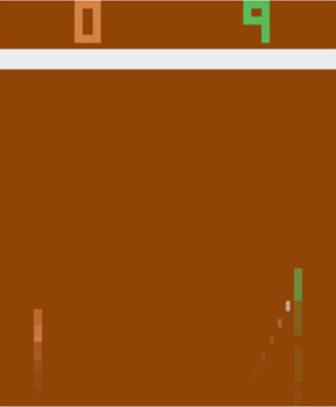
\includegraphics[width=\textwidth]
            {figures/explainability_in_reinforcement_learning/policy_approximation_observation.jpg}
        \caption{}
        \label{fig:policy_approximation_observation}
    \end{subfigure}
    \hspace{0.02\textwidth}
    \begin{subfigure}[b]{0.47\textwidth}
        \centering
        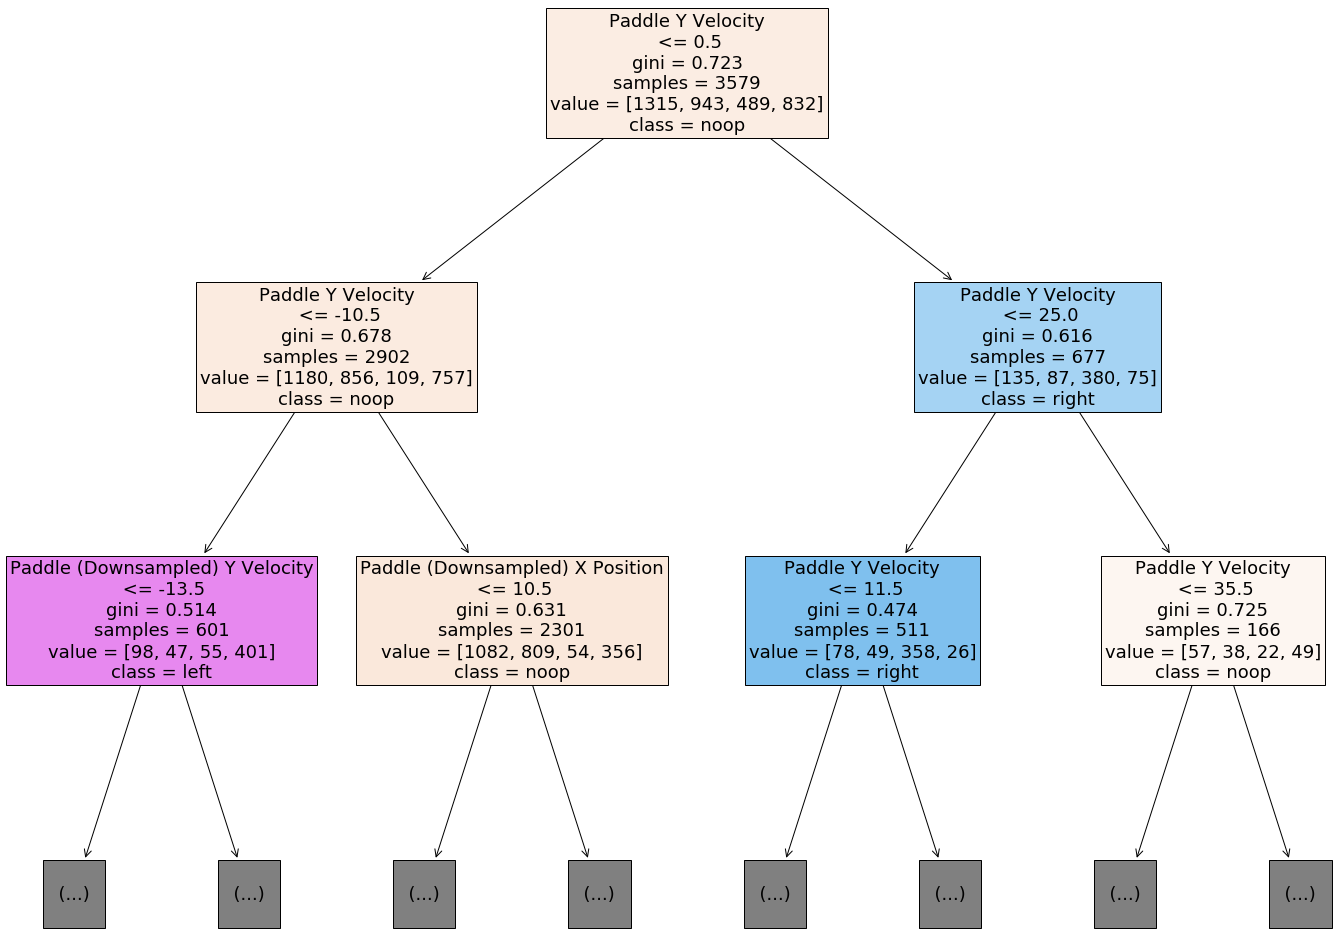
\includegraphics[width=\textwidth]
            {figures/explainability_in_reinforcement_learning/policy_approximation_decision_tree.png}
        \caption{}
        \label{fig:policy_approximation_decision_tree}
    \end{subfigure}
    \caption[Policy approximation via an interpretable model.]{
        Policy approximation via an interpretable model \parencite{sieusahai2021explaining}.
    }
    \label{fig:policy_approximation_example}
\end{figure}


\subsection{Saliency Map}
\label{subsec:saliency_map}

The influence of each part of the input on the action selected by the policy can be visualized using heatmaps (Figure~\ref{fig:saliency_map_heatmap}).
In the \gls{rl} setting, the input corresponds to the observation received by the agent at a given time step.
Heatmaps therefore highlight the regions of the observation that have the greatest influence on the action selection process.
By providing this information, they allow the observer to identify which elements of the environment are considered important by the policy when making a decision.
In Figure~\ref{fig:saliency_map_heatmap}, both panels correspond to the same observation of the Atari game \BreakoutName, with panel~\subref{fig:saliency_map_heatmap_perturbation} obtained by observation perturbation and panel~\subref{fig:saliency_map_heatmap_gradient} by observation gradient analysis.

\begin{figure}[t]
    \centering
    \begin{subfigure}[b]{0.4\textwidth}
        \centering
        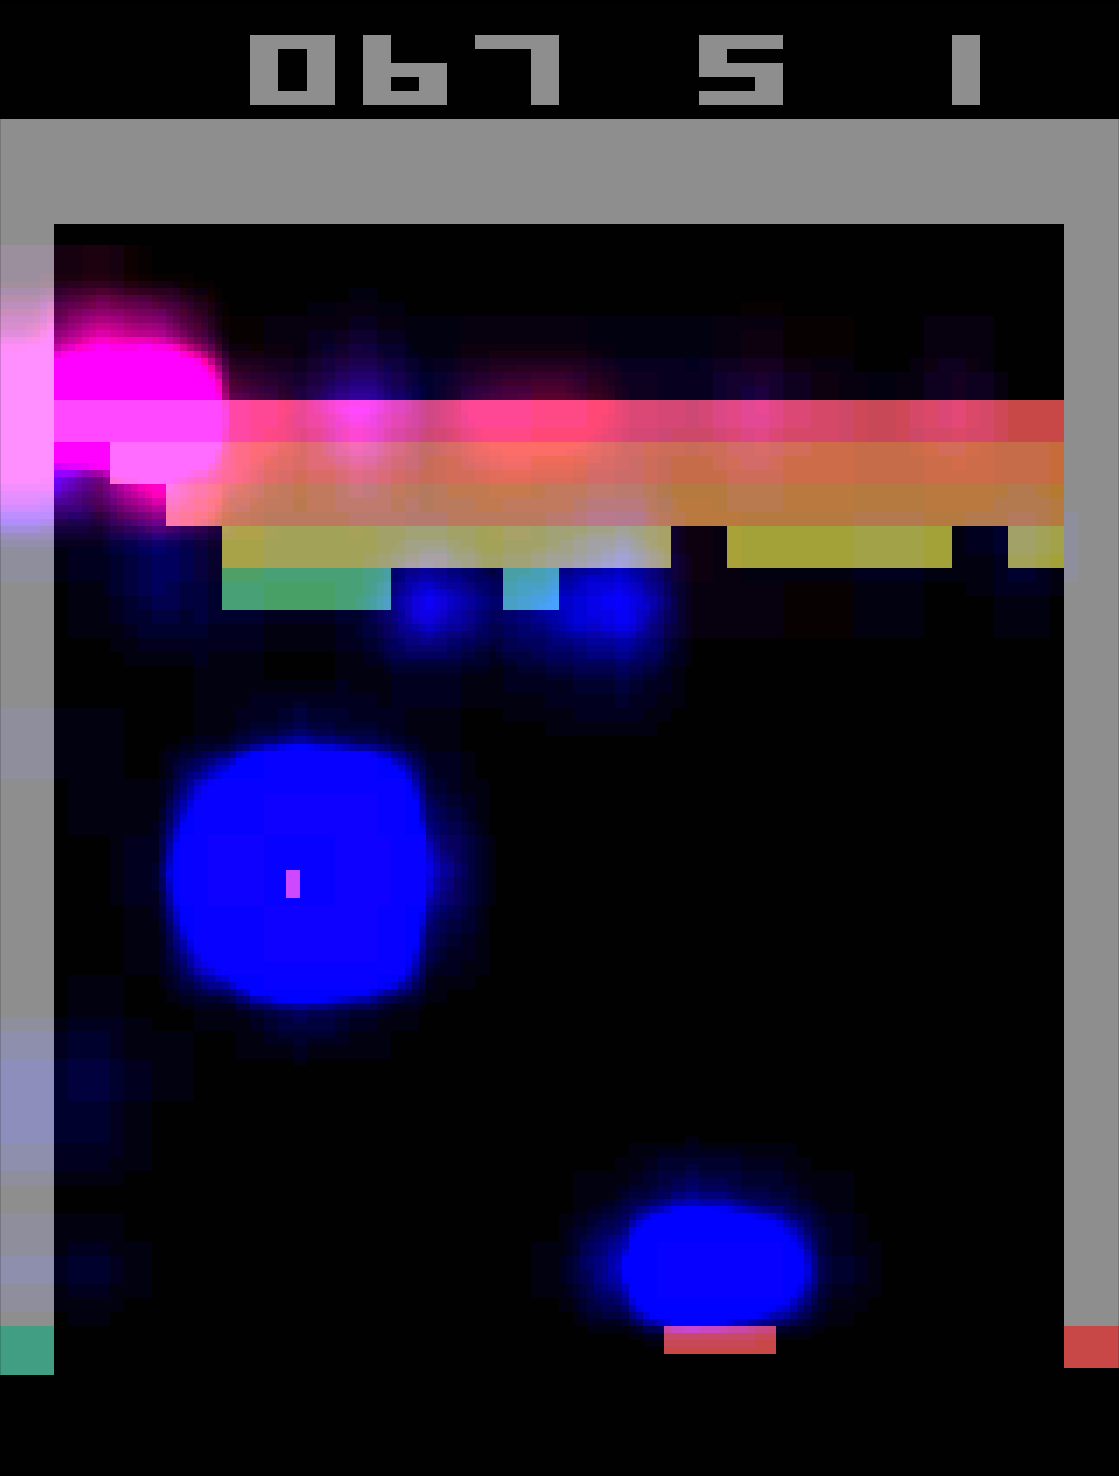
\includegraphics[width=\textwidth]
            {figures/explainability_in_reinforcement_learning/hit_map_1.png}
        \caption{}
        \label{fig:saliency_map_heatmap_perturbation}
    \end{subfigure}
    \hspace{0.02\textwidth}
    \begin{subfigure}[b]{0.4\textwidth}
        \centering
        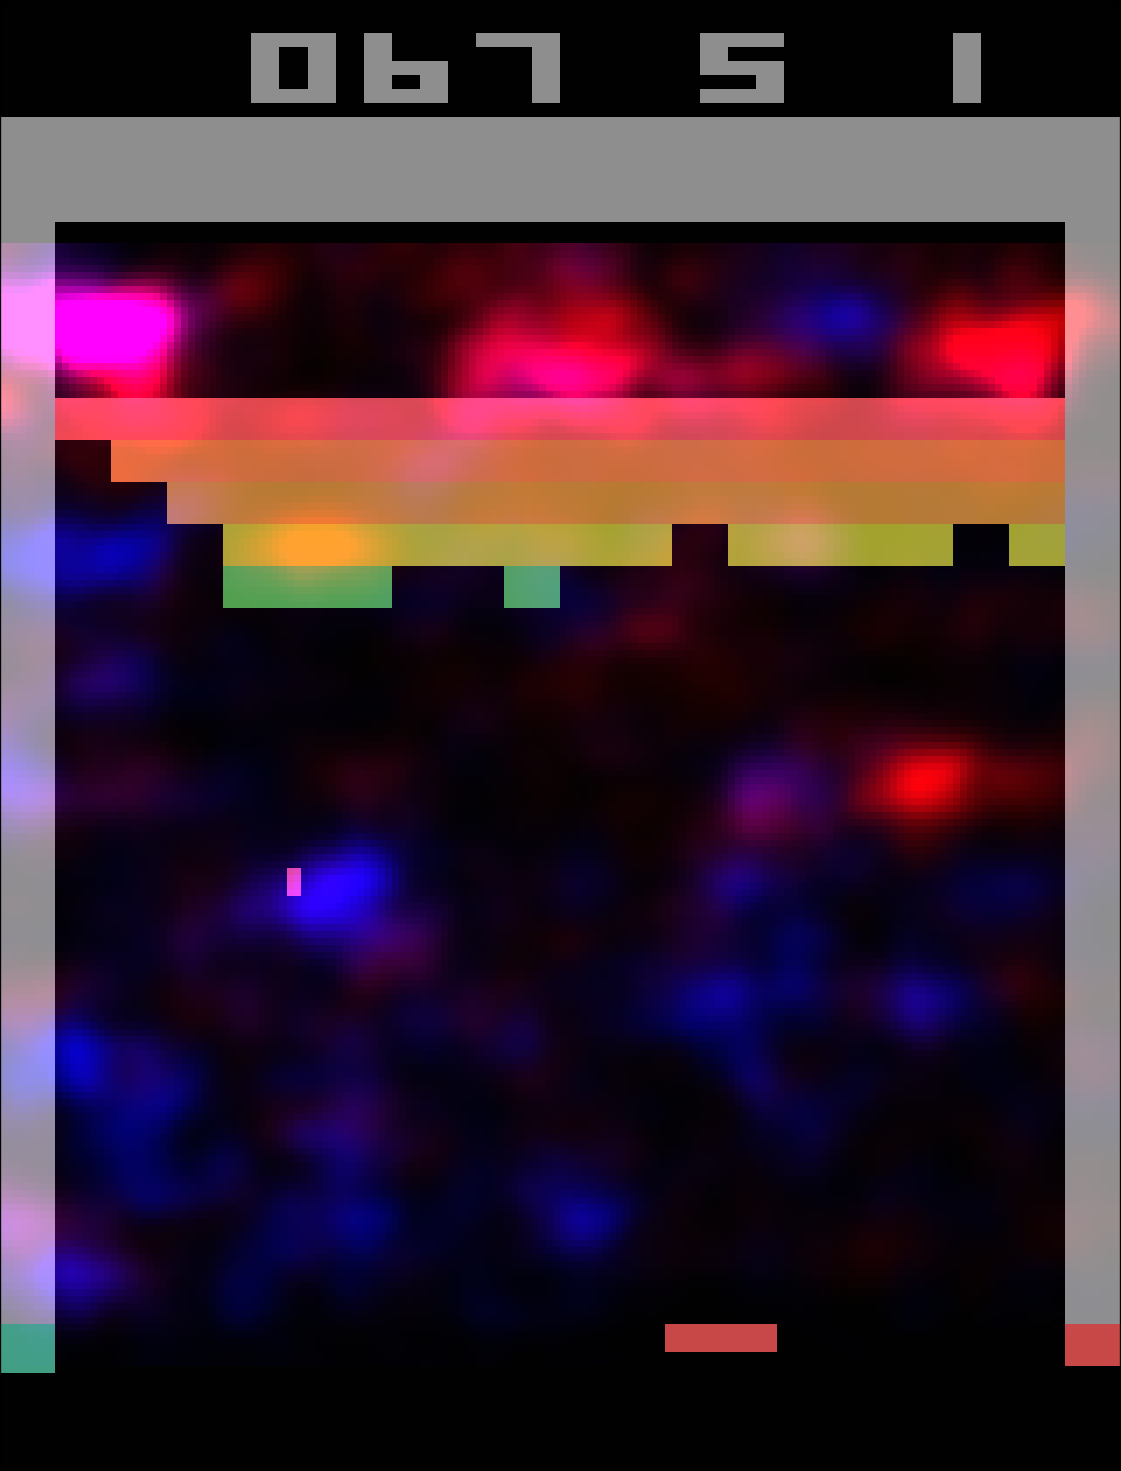
\includegraphics[width=\textwidth]
            {figures/explainability_in_reinforcement_learning/hit_map_2.png}
        \caption{}
        \label{fig:saliency_map_heatmap_gradient}
    \end{subfigure}
    \caption[Saliency heatmaps for \BreakoutName.]{
        Heatmaps for the same observation of the Atari game \BreakoutName \parencite{greydanus2018visualizing}.
    }
    \label{fig:saliency_map_heatmap}
\end{figure}


A limitation of heatmap-based methods is that the resulting explanations are not always directly meaningful to the observer.
As illustrated in Figure~\ref{fig:saliency_map_heatmap_gradient}, interpreting which regions are important often requires human reasoning and involves a degree of subjectivity.
This limitation becomes particularly relevant in \gls{rl}, where the objective is not only to explain a single decision but also to understand the factors influencing a sequence of decisions over time.

Three families of explainability methods can be used to obtain this type of explanation: \textit{observation perturbation}, \textit{observation gradient analysis}, and \textit{attention-based architectures}.

\subsubsection{\textit{Observation Perturbation}}
\label{subsubsec:observation_perturbation}

Perturbation analysis consists in applying various modifications to the observation in order to study their impact on the output of the policy function \parencite{greydanus2018visualizing}.
The greater the variation in the output caused by a perturbation applied to a given component of the input vector, the higher the weight assigned to that component.
The magnitude of the perturbation is measured by computing the distance between the original output and the output obtained from the perturbed input.
Using this set of weights, a \textit{heatmap} is constructed, enabling the observer to visualize which parts of the observation vector are most sensitive in the action-selection process (see Figure~\ref{fig:saliency_map_heatmap_perturbation}).

\subsubsection{\textit{Observation Gradient Analysis}}
\label{subsubsec:observation_gradient_analysis}

Observation gradient analysis refers to a set of methods that require a differentiable policy function in order to extract information from it \parencite{simonyan2014deep, weitkamp2019visual, huber2019enhancing}.
To this end, the gradient of the policy function is computed with respect to all components of the input vector.
For each input component, the resulting gradient provides a weighting that represents its importance in the output of the policy function.
Based on these weightings, a \textit{heatmap} is constructed to allow the observer to visually identify the parts of the input vector that are the most influential in the policy function's output (see Figure~\ref{fig:saliency_map_heatmap_gradient}).

\subsubsection{\textit{Attention-Based Architecture}}
\label{subsubsec:attention_based_architecture}

Attention blocks constitute a \gls{nn} architecture that makes it possible to weight the relative importance of one part of a vector with respect to the other parts of the same vector \parencite{vaswani2017attention}.
These weights are computed as a function of the vector itself and are learned by the \gls{nn} during training.
For a given observation, each component of the observation vector is assigned a scalar value.
It can therefore be assumed that the components associated with the highest weights are the most influential in determining the output \parencite{mott2019towards, itaya2021visual}.

This attention-based \textit{heatmap} is then provided to the observer as the explanation, as illustrated for the Atari game \BreakoutName in Figure~\ref{fig:attention_map_heatmap_clear}, where the highlighted regions are easily interpretable.
However, as shown for \MsPacManName in Figure~\ref{fig:attention_map_heatmap_unclear}, the attention weights are not always concentrated on a small, easily interpretable set of regions, which can make this type of explanation difficult to exploit.

\begin{figure}[t]
    \centering
    \begin{subfigure}[b]{0.4\textwidth}
        \centering
        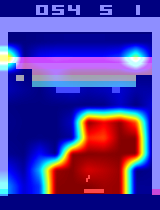
\includegraphics[width=\textwidth]
            {figures/explainability_in_reinforcement_learning/attention_map_1.png}
        \caption{}
        \label{fig:attention_map_heatmap_clear}
    \end{subfigure}
    \hspace{0.02\textwidth}
    \begin{subfigure}[b]{0.4\textwidth}
        \centering
        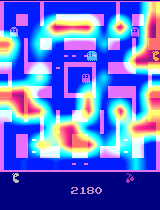
\includegraphics[width=\textwidth]
            {figures/explainability_in_reinforcement_learning/attention_map_2.png}
        \caption{}
        \label{fig:attention_map_heatmap_unclear}
    \end{subfigure}
    \caption[Attention-based heatmaps for \BreakoutName and \MsPacManName.]{
        Attention-based heatmaps for the Atari games \BreakoutName and \MsPacManName \parencite{mott2019towards}.
    }
    \label{fig:attention_map_heatmap}
\end{figure}


\subsection{Counterfactual}
\label{subsec:counterfactual}

A counterfactual explanation is a new observation, close to the original one, that leads the agent to select a different action.
Comparing the two observations reveals which elements of the environment must change for the agent to behave differently, and thus provides insight into its decision-making process.
Unlike the other forms of explanation, this form is currently associated with a single family of methods, based on the \textit{use of the \gls{ls} for counterfactual generation}.

\subsubsection*{\textit{Latent Space Usage for Counterfactual Generation}}
\phantomsection\label{subsubsec:latent_space_counterfactual_generation}

This family of methods uses generative models to build counterfactuals from the \gls{lr} of the observation \parencite{bond2021deep, olson2021counterfactual}.
The observation is encoded into the \gls{ls}, its representation is modified until the agent selects the desired action, and this modified representation is decoded back into a new observation.
Working in the \gls{ls} rather than at the pixel level keeps the counterfactual close to the original state and consistent with the environment.
The fidelity of the generated observations to the real game can then be assessed through user studies \parencite{olson2021counterfactual}.

Figure~\ref{fig:counterfactual_example} illustrates this approach on the Atari game \SpaceInvadersName \parencite{olson2021counterfactual}.
In the original observation (Figure~\ref{fig:counterfactual_example_original}) the agent selects \texttt{LEFT}, whereas in the counterfactual observation (Figure~\ref{fig:counterfactual_example_counterfactual}) it selects \texttt{RIGHT\_FIRE}.
Here, removing an enemy is enough to change the action, which suggests that the position of that enemy influences the agent's decision.
Such observations remain only indicative. Identifying a reliable pattern requires repeating the analysis across many situations.

\begin{figure}[t]
    \centering
    \begin{subfigure}[b]{0.35\textwidth}
        \centering
        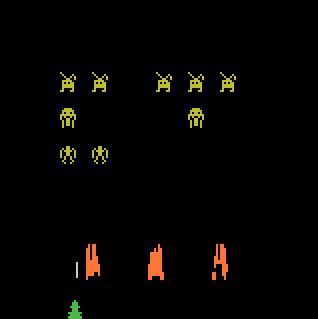
\includegraphics[width=\textwidth]
            {figures/explainability_in_reinforcement_learning/contrefactuel_1.png}
        \caption{}
        \label{fig:counterfactual_example_original}
    \end{subfigure}
    \hspace{0.02\textwidth}
    \begin{subfigure}[b]{0.35\textwidth}
        \centering
        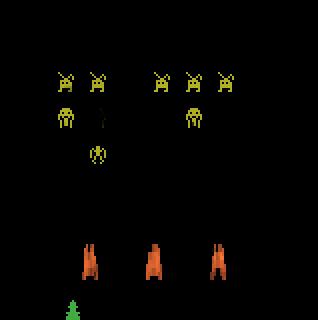
\includegraphics[width=\textwidth]
            {figures/explainability_in_reinforcement_learning/contrefactuel_2.png}
        \caption{}
        \label{fig:counterfactual_example_counterfactual}
    \end{subfigure}
    \caption[Counterfactual explanation for \SpaceInvadersName.]{
        Counterfactual explanation of the agent's behavior for the Atari game \textit{\SpaceInvadersName} \parencite{olson2021counterfactual}.
        Panel~\subref{fig:counterfactual_example_original} shows the original observation and panel~\subref{fig:counterfactual_example_counterfactual} the counterfactual observation produced by a generative model.
    }
    \label{fig:counterfactual_example}
\end{figure}


\subsection{Agent Trajectory}
\label{subsec:agent_trajectory}

Until now, the presented methods have focused on explaining individual decisions made by the agent.
The methods considered from this point on aim to provide insight into the agent's strategy by analyzing its behavior over time.

The most direct approach consists in visualizing agent trajectories, most commonly through complete episodes.
By analyzing these trajectories, the observer can infer the dynamics underlying the agent's behavior and how its decisions evolve through time.
This type of visualization is not specific to \gls{xrl}.
In practice, visualizing agent episodes is a standard step in the development and evaluation of \gls{rl}.
It provides a simple way to verify that the agent behaves as expected and to detect potential implementation errors.

This simple approach can be further enhanced using families of methods such as \textit{hierarchical decomposition} and \textit{extraction via critic analysis}.

\subsubsection{\textit{Extraction via Critic Analysis}}
\label{subsubsec:extraction_via_critic_analysis}

In this family of methods, the predictions of the critic are used to determine which trajectories to present to the observer \parencite{Sequeira_2020}.
A set of states is selected from multiple trajectories.
For a given state, all possible actions are examined.
The state is assigned a value equal to the difference between the critic's prediction for the lowest-valued action and the prediction for the highest-valued action.

Trajectories containing the states with the highest values according to this procedure are then chosen to be presented to the observer.
These trajectories are considered critical moments of the agent and are therefore relevant for analysis.
For this family of methods, the \textit{selected trajectories} represent the interpretable information provided to the observer.

\subsubsection{\textit{Hierarchical Decomposition}}
\label{subsubsec:hierarchical_decomposition}

Hierarchical agents are composed of a set of sub-policies specialized for specific tasks within subsets of the environment's states.
This family of methods distributes the optimization of the reward function across multiple policies.
This decomposition of the policy function can also provide explainability in the agent's strategy \parencite{Beyret_2019}.

If a sub-policy is selected, it indicates that the agent will execute a specialized behavior.
This behavioral specialization provides insight into the strategy the agent employs to maximize the reward function.
The agent's \textit{trajectory}, together with the \textit{sub-policy} selected for each action, is used as interpretable information.

\subsection{Trajectory Prediction}
\label{subsec:trajectory_prediction}

Making predictions about the future of a trajectory allows one to form a representation of what the system expects, based on its training experience.
These predictions are produced using value functions.
Such functions provide insights into the future evolution of the agent's trajectory.
By their nature, this form of explanation informs the observer about the strategy adopted by the agent.

Value functions provide an estimate of the expected cumulative reward from a given state.
Consequently, a value function maps an observation to a scalar value in $\mathbb{R}$.
This aggregated prediction provides limited information about the underlying factors that contribute to this value.
It does not directly reveal which aspects of the task are being optimized or how the predicted return is composed.
Unlike the other forms of explanation, this form is currently associated with a single family of methods, aimed at improving the interpretability of value-based explanations: \textit{critic enrichment}.

\subsubsection*{\textit{Critic Enrichment}}
\phantomsection\label{subsubsec:critic_enrichment}

In order to obtain interpretable information from the predictions of the critic, it is possible to decompose the critic into multiple sub-functions \parencite{juozapaitis2019explainable}.
The reward function is thus decomposed into multiple sub-reward functions, each representing a sub-objective of the task to be accomplished.
Similarly, for each of these sub-reward functions, corresponding sub-critic functions are defined, along with a function that combines their outputs.
During training, the agent selects its actions so as to maximize this combination function of the sub-critics.

Using this approach, for each observation and action, a prediction is obtained regarding the sub-objectives the agent is attempting to maximize, so that the action chosen by the agent reveals which sub-reward it aims to maximize (see Figure~\ref{fig:trajectory_prediction_values}).
This \textit{prediction} is then used as the explanation for the observer.

\begin{figure}[t]
    \centering
    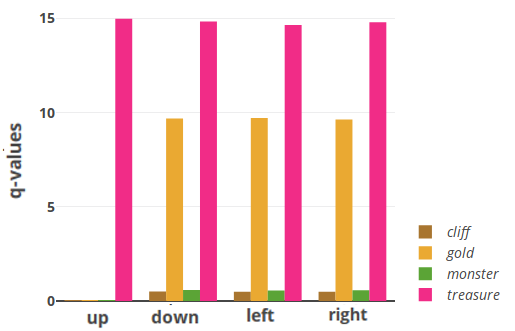
\includegraphics[width=0.8\textwidth]
        {figures/explainability_in_reinforcement_learning/multi_q_values.png}
    \caption[Prediction of sub-rewards as a function of the selected action.]{
        Prediction of sub-rewards as a function of the action selected by the agent for a given state \parencite{juozapaitis2019explainable}.
    }
    \label{fig:trajectory_prediction_values}
\end{figure}


\subsection{Interaction Model}
\label{subsec:interaction_model}

Modeling the interactions between an agent and its environment makes it possible to understand how the agent's decisions are made and what impact they have on the environment.
By incorporating these interactions into an explanatory model, one can better grasp the complex relationships between the agent and its environment, thereby identifying the determining factors in the decision-making process.
By explicitly handling the agent--environment interaction, this type of explanation aims to explain the agent's strategy.

The families of methods used to obtain explanations in the form of agent--environment interactions are: \textit{Bayesian network learning} and \textit{\gls{ls} usage for \gls{mdp} generation}.

\subsubsection{\textit{Bayesian Network Learning}}
\label{subsubsec:bayesian_network_learning}

The evolution of an agent within an environment can be observed as a set of random variables connected through a Bayesian network \parencite{madumal2020explainable}.
Random variables are defined to represent both external aspects (the environment) and internal aspects of the agent (the actions).
By analyzing trajectories, it becomes possible to infer causal relationships among these random variables.

At the end of this process, a weighted causal graph is obtained, which serves as an explanation for the observer, as illustrated for the video game \StarCraftIIName in Figure~\ref{fig:interaction_model_causal_graph}, where nodes represent random variables and edges represent causal relationships between them.
This \textit{Bayesian network}, representing the interactions between the agent and the environment, is then used as the explanation.

\begin{figure}[t]
    \centering
    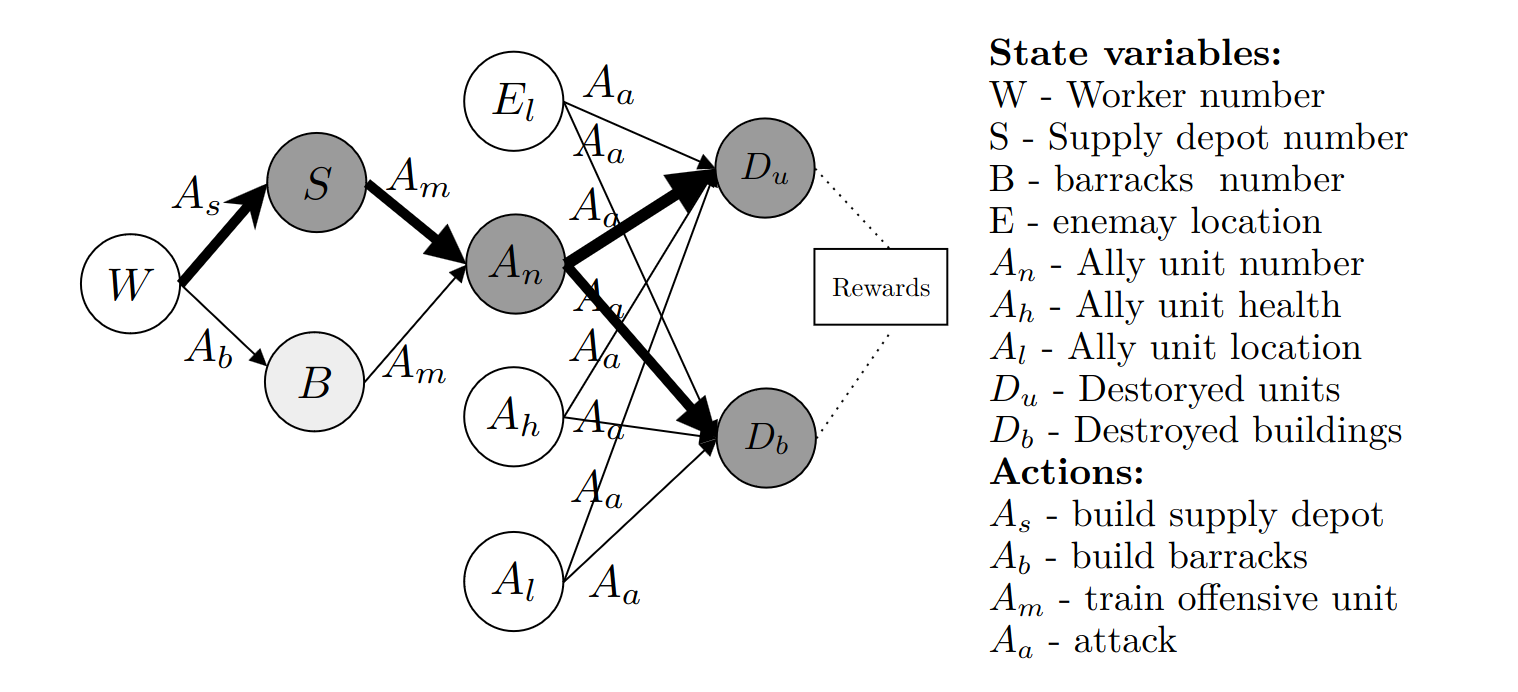
\includegraphics[width=0.9\textwidth]
        {figures/explainability_in_reinforcement_learning/graph_causal.png}
    \caption[Agent--environment interaction model for \StarCraftIIName.]{
        Agent--environment interaction model for the video game \StarCraftIIName \parencite{madumal2020explainable}.
    }
    \label{fig:interaction_model_causal_graph}
\end{figure}


\subsubsection{\textit{Latent Space Usage for Markov Decision Process Generation}}
\label{subsubsec:latent_space_mdp_generation}

As discussed in Chapter~\ref{chap:latent_space_analysis}, each layer of a \gls{nn} can be viewed as a projection from one space to another \parencite{zahavy2017graying}.
As information propagates through successive layers of a \gls{nn}, it becomes increasingly abstract.
It can therefore be assumed that two vectors that are close in this projected space are also close in terms of the agent's perception.

Based on this observation, it is possible to redefine an \gls{mdp} by leveraging the abstract representations produced by the final layers of a \gls{nn}.
Once the new \gls{mdp} has been constructed, a model of the interaction between the agent and its environment is obtained.
This model, represented as a \textit{graph}, is then used as the explanation.

Figure~\ref{fig:latent_space_tsne_example} illustrates this idea using a two-dimensional \textit{t-SNE} projection of the \gls{ls} of the \gls{nn} used to represent the policy.
Each point is colored according to the value function's prediction for the corresponding state, with warmer colors indicating higher predicted values.
An agreement can be observed between the structure of this projected space and the critic's predictions.
States that are assigned similar values by the critic also tend to be located close to one another in the projection.
This agreement makes it possible to manually identify clusters of states, which likely correspond to states that are perceived as similar by the agent.

\begin{figure}[t]
    \centering
    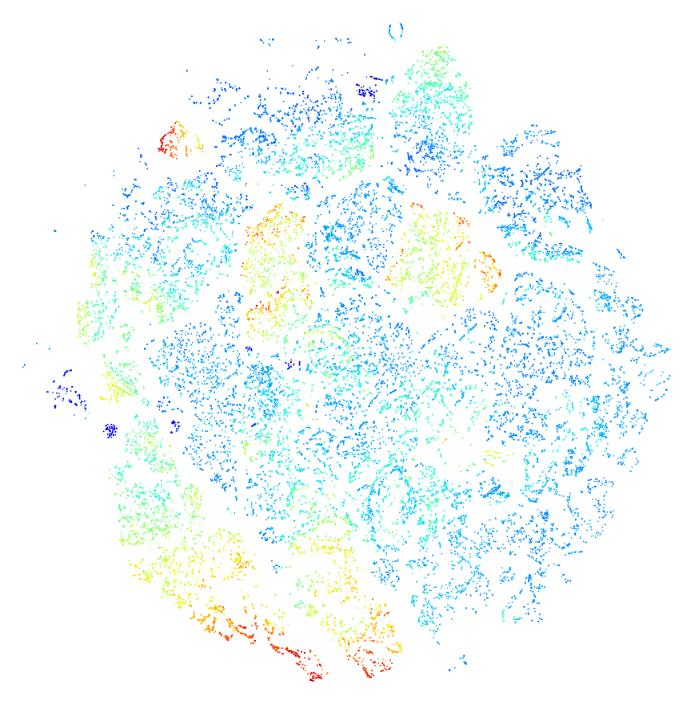
\includegraphics[width=0.8\textwidth]
        {figures/explainability_in_reinforcement_learning/latent_space_tsne_value_function.jpg}
    \caption[\textit{t-SNE} projection of an \glsfmtshort{nn}'s \glsfmtshort{ls}.]{
        \textit{t-SNE} projection of an \glsfmtshort{nn}'s \glsfmtshort{ls}
        \parencite{zahavy2017graying}.
    }
    \label{fig:latent_space_tsne_example}
\end{figure}


\section{Conclusion}
\label{sec:explainability_in_reinforcement_learning_conclusion}

The taxonomy and the state-of-the-art review presented in this chapter make it possible to draw three main observations.

\subsection{Absence of Explanation of the Learning Process}

Regarding the subject of explanation, Table~\ref{tab:taxonomy_methods} shows that none of the reviewed methods addresses the learning process itself.
Such an explanation would concern how the policy is progressively updated throughout training, and why it evolves over successive iterations to converge toward a particular solution.
Several reasons explain this absence.

First, among the different machine learning paradigms, \gls{rl} is arguably the one that would benefit the most from explanations of the learning process.
Unlike supervised or unsupervised learning, it relies on an explicit exploration--exploitation trade-off, making the learning trajectory itself an informative subject of explanation.
However, most \gls{xrl} methods are inherited from the XAI literature, where explanations focus exclusively on the behavior of already-trained models.
This limitation has naturally carried over to \gls{xrl}.

Second, explanations of the learning process have limited value from a practical perspective.
In most real-world applications, practitioners deploy an already-trained agent.
Practitioners are therefore primarily interested in understanding the behavior of the final policy rather than the optimization process that produced it.

Finally, explaining the learning process raises significant methodological challenges.
Training in \gls{rl} can be viewed as the iterative improvement of a policy through repeated interactions with the environment.
In this sense, explaining learning would amount to explaining the evolution of an entire sequence of policies rather than a single one.
Current \gls{xrl} methods still struggle to provide comprehensive explanations of an individual policy, so extending them to a full training trajectory appears considerably more difficult.

\subsection{Lack of Unified Metrics for Explainability}

The diversity of explanation forms identified in this review also reveals another limitation shared by nearly all families of \gls{xrl} methods, which is the absence of reliable metrics for evaluating explainability.
In many studies, explanations are not evaluated with human participants.
Instead, authors focus on technical properties of the proposed method, such as fidelity, sparsity, or computational efficiency.

When human evaluations are conducted, they usually rely on subjective satisfaction questionnaires.
Although useful, self-reported satisfaction remains prone to numerous biases and does not necessarily indicate that the explanation has improved the observer's mental model or understanding of the agent.

This limitation is not specific to \gls{xrl}, it reflects a broader challenge affecting \gls{xai} as a whole.
In our view, this limitation comes from how explainability has developed in artificial intelligence.
Most of the proposed approaches have been developed by the computer science community.
Explainability has consequently often been studied from an algorithmic or mathematical perspective, with less attention given to how humans actually benefit from explanations.

Our definition of explanation explicitly places the observer at the center of the explanatory process.
From this perspective, the value of an explanation should not only depend on its technical properties but also on its ability to improve the observer's understanding.
Addressing this challenge will require stronger interdisciplinary collaboration between computer science and disciplines such as cognitive science, psychology, philosophy, and sociology.
These fields provide the theoretical and experimental tools needed to study human understanding and to develop evaluation protocols that measure the actual effectiveness of explanations.

\subsection{Toward Intrinsic Explainability in Reinforcement Learning}

Our review also suggests that current \gls{xrl} research remains largely dominated by substitutive explainability approaches.
Replacing a deep model with a simpler one therefore risks losing precisely the representational power that makes deep \gls{rl} effective.
For this reason, we argue that a promising direction for \gls{xrl} is to develop explanations directly from the \gls{nn} that forms the agent's policy.
Such approaches aim to analyze the representations learned by the network itself.

Among the methods reviewed, \textit{latent space usage for MDP generation} (Section~\ref{subsubsec:latent_space_mdp_generation}) appears closest to this intrinsic perspective.
However, this approach still relies on a largely manual and qualitative analysis of the \gls{ls}, which limits its reproducibility and its ability to produce systematic explanations.

The next chapter builds upon this idea and proposes a mechanistic \gls{xrl} approach based on \gls{ls} analysis.
